%%% LaTeX Template: Two column article
%%%
%%% Source: http://www.howtotex.com/
%%% Feel free to distribute this template, but please keep to referal to http://www.howtotex.com/ here.
%%% Date: February 2011

%%% Preamble
\documentclass[	DIV=calc,%
							paper=a4,%
							fontsize=12pt,%
							onecolumn]{scrartcl}	 					% KOMA-article class

\usepackage{lipsum}													% Package to create dummy text
\usepackage[brazil]{babel}										% English language/hyphenation
\usepackage[protrusion=true,expansion=true]{microtype}				% Better typography
\usepackage{amsmath,amsfonts,amsthm}					% Math packages
\usepackage[pdftex]{graphicx}									% Enable pdflatex
\usepackage[svgnames]{xcolor}									% Enabling colors by their 'svgnames'
\usepackage[hang, small,labelfont=bf,up,textfont=it,up]{caption}	% Custom captions under/above floats
\usepackage{epstopdf}												% Converts .eps to .pdf
\usepackage{subfig}													% Subfigures
\usepackage{booktabs}												% Nicer tables
\usepackage{fix-cm}													% Custom fontsizes
\usepackage[utf8]{inputenc}
\usepackage[top=2.5cm, bottom=2.5cm, left=2.5cm, right=2.5cm]{geometry}
\usepackage[ddmmyyyy]{datetime}
\usepackage{gensymb}
\usepackage{textcomp}
\addto\captionsenglish{%
	\renewcommand\tablename{Tabela}
	\renewcommand\figurename{Figura}
} 
 

 
%%% Custom sectioning (sectsty package)
\usepackage{sectsty}													% Custom sectioning (see below)
\allsectionsfont{%															% Change font of al section commands
	\usefont{OT1}{phv}{b}{n}%										% bch-b-n: CharterBT-Bold font
	}

\sectionfont{%																% Change font of \section command
	\usefont{OT1}{phv}{b}{n}%										% bch-b-n: CharterBT-Bold font
	}



%%% Headers and footers
\usepackage{fancyhdr}												% Needed to define custom headers/footers
	\pagestyle{fancy}														% Enabling the custom headers/footers
\usepackage{lastpage}	

% Header (empty)
\lhead{}
\chead{}
\rhead{}
% Footer (you may change this to your own needs)

%% ====================================
%% ====================================
%% mude o rodape  do projeto
%% ====================================
%% ====================================

\lfoot{\footnotesize \texttt{Cabeamento estruturado} \textbullet ~Modelo de projeto}


\cfoot{}
\rfoot{\footnotesize página \thepage\ de \pageref{LastPage}}	% "Page 1 of 2"
\renewcommand{\headrulewidth}{0.0pt}
\renewcommand{\footrulewidth}{0.4pt}



%%% Creating an initial of the very first character of the content
\usepackage{lettrine}
\newcommand{\initial}[1]{%
     \lettrine[lines=3,lhang=0.3,nindent=0em]{
     				\color{DarkGoldenrod}
     				{\textsf{#1}}}{}}



%%% Title, author and date metadata
\usepackage{titling}															% For custom titles

\newcommand{\HorRule}{\color{DarkGoldenrod}%			% Creating a horizontal rule
									  	\rule{\linewidth}{1pt}%
										}

\pretitle{\vspace{-30pt} \begin{flushleft} \HorRule 
				\fontsize{50}{50} \usefont{OT1}{phv}{b}{n} \color{DarkRed} \selectfont 
				}

%% ====================================
%% ====================================
%% mude o titulo  do projeto
%% ====================================
%% ====================================

\title{Modernização e Organização de Cabos Unimed-Foz}					% Title of your article goes here

%% ====================================



\posttitle{\par\end{flushleft}\vskip 0.5em}

\preauthor{\begin{flushleft}
					\large \lineskip 0.5em \usefont{OT1}{phv}{b}{sl} \color{DarkRed}}
\author{Jeverson Siqueira}  	% Author name goes here


\postauthor{\footnotesize \usefont{OT1}{phv}{m}{sl} \color{Black} 
					\\Universidade Tecnológica Federal do Paraná - Câmpus Cornélio Procópio 								% Institution of author
					\par\end{flushleft}\HorRule}

\date{}																				% No date




%%% Begin document
\begin{document}
\maketitle
\thispagestyle{fancy} 	
\thispagestyle{empty}		% Enabling the custom headers/footers for the first page 
% The first character should be within \initial{}




%% ====================================
%% ====================================
%% mude o resumo  do projeto
%% ====================================
%% ====================================
\initial{E}\textbf{
	Este projeto visa a modernização, organização dos cabos atuais no data center da Unimed Foz do Iguaçu, isso ira prover redução de erros na camada física, facilidade em encontrar erros na camada física, crescimento organizado, escalabilidade, segmentação modular da camada física e manutenção em setores. Todos os dados aqui levantados serão fictícios para a realização desse trabalho, mas será levantado como base alguns dados reais, que serão descritos no decorrer desse projeto. 
}

%% ====================================
\begin{figure}
	\centering
	
\includegraphics{utfpr}
\end{figure}

\vspace{3cm}
\centerline{\textit{\textbf{\today}}}





\clearpage
\renewcommand{\contentsname}{Sumário}
\tableofcontents
\clearpage

%% ====================================
%% ====================================
%% Inicio do texto
%% ====================================
%% ====================================
\section{Introdução}

A atual Unimed localizada no centro de Foz do Iguaçu conta com 40 colaboradores em sua sede administrativa, e no hospital conta com mais 100 colaboradores. Cada uma das Unimed possui seu próprio data center com isso iremos aplicar primeiramente na sede onde possui um parque de máquinas menores comparadas ao hospital. Atualmente na Unimed sede contamos com 45 equipamentos para uso dos funcionários, no data center contamos com um Storage de backup diário, um servidor mais completo para virtualizações onde nele conta com as virtualizações do LDAP (Lightweight Directory Access Protocol), servidor Web, Firewall e Proxy. As demais aplicações que os usuários usam são software normais do dia-a-dia como e-mail, edição de arquivos de textos e sistemas voltados para saúde etc. Esse documento será aplicado no data center para melhorar primeiro a sua estrutura, as demais equipamentos serão atualizados os cabos de rede, para assim manter um padrão adequados entre eles.

\subsection{Benefícios}
Os benefícios que teria após a execução desse projeto serias várias tais como: 

\begin{itemize}
	\item Redução de erros na camada física;
	\item facilidade em encontrar erros na camada física;
	\item crescimento organizado;
	\item escalabilidade;
	\item segmentação modular da camada física;
	\item manutenção em setores.
\end{itemize}
 
\subsection{Organizações Envolvidas}
A atual organização envolvida é a Unimed sede administrativa, ainda existe o Hospital que já é outro cenário tendo mais computadores e colaboradores, os servidores lotados no Unimed administrativo possui as mesmas funções do que no hospital, sendo uma AD, Proxy, Firewall e um para sistema de arquivos. No entanto não será levantado um cenário em comparação entre os dois. Talvez isso seja em algum outro trabalho futuro.


\section{Requisitos}\label{sec:Requisitos}
Os requisitos coletados para implantação levantados verificando as estrutura atual do data center podem ser visto na tabela \ref{tab:requisitos}.

\begin{table}[!htbp]
	\centering
	\begin{tabular}{|l|l|ll}
		\cline{1-2}
		\textbf{Componentes}        & \textbf{Qts.} &  &   \\
		\cline{1-2}
		Patch panel (furukawa GIGALAN CAT.6 de 24 portas) & 4    &  &   \\
		Switch gerenciável (Cisco 2960L ) & 2    &  &   \\
		Access Points 	   (Cisco Air-lap 1141n-a-k) & 4    &  &   \\
		Servidor Monitoramento SNMP 	   & 1    &  &   \\	
		Patch Cord Cat.6  1m	   & 72    &  &   \\
		Patch Cord Cat.6  5m	   & 72    &  &   \\
		Fluke Microscanner2	   & 1    &  &   \\
		\cline{1-2} 
	\end{tabular}
		\caption{Tabela para requisitos do projeto}\label{tab:requisitos}
\end{table}


\section{Usuários e Aplicativos}
A quantidade atual de usuário na Unimed sede são de 40 colaboradores, a estimativa de evolução é de pouco colaboradores devido as demandas da empresa, pensado nisso na seção \ref{sec:Requisitos} foram devidos mais estrutura do que atual, pensado já no crescimento de equipamentos e usuários na rede, assim como pontos de redes necessários. 

\subsection{Usuários}
	A seguir pode ser conferido na tabela \ref{tab:usuarios} a quantidade de usuários, juntamente com seus perfil de acesso:
	\begin{table}[!htbp]
		\centering
		\begin{tabular}{|l|l|ll} 
			\cline{1-2}
			\textbf{Usuários}                                  & \textbf{Perfil de acessos} &  &   \\ 
			\cline{1-2}
			Usuário Comuns                                     & 45                         &  &   \\
			Usuário Administradores                            & 2                          &  &   \\
			Usuários VPN                                       & 3                          &  &   \\
			Usuários Para Demais aplicações (Antivírus, Roots) & 5                          &  &   \\
			\cline{1-2}
		\end{tabular}
		\caption{Tabela com perfis de usuários}\label{tab:usuarios}
	\end{table}

\subsection{Aplicativos}
Aqui são demostrados as aplicações dos usuário e críticas do projeto, alguma aplicações são críticas dependendo de sua utilidades ou setor, por exemplo setores como financeiro e perícia médica devem serem alojados em Vlans específicas e manter uma certa prioridade em relação dos backup individuais de cada equipamento. 

\begin{table}[!htbp]
	\centering
	\resizebox{\textwidth}{!}{\begin{tabular}{|l|l|l|l} 
		\cline{1-3}
		\textbf{Setor} & \textbf{Nível de complexidade} & \textbf{Aplicações}                                                        &   \\ 
		\cline{1-3}
		RH             & Média                          & Aplicações de Cartão Ponto, E-mail e edição de textos~                     &   \\ 
		\cline{1-3}
		Liberação~     & Alta                           & Aplicações de liberações de exames, E-mail, edição de texto                &   \\
		\cline{1-3}
		SAC            & Baixa                          & Aplicações de texto, e-mail                                                &   \\
		\cline{1-3}
		Cadastro       & Média                          & Criação de contas e planos, E-mail, edição de textos                       &   \\
		\cline{1-3}
		Comercial      & Média                          & Software de Design e market, acesso a redes socias, e-mail edição de texto &   \\
		\cline{1-3}
		TI       	   & Alta                           & Gerenciamento de usuários, Datacenter, todo funcionamento dos softwares   &   \\
		\cline{1-3}
	\end{tabular}}
	\caption{Aplicações e nível de complexidade dos usuários}\label{tab:aplicacoes}
\end{table}


\section{Estrutura predial existente}
A estrutura da sala do data center junto com as distâncias dos cabos e servidores são descritas em imagens para o melhor entendimento do projeto, será apresentada a descrição junto com a topologia aplicada na sala.

\section{Planta Lógica - Elementos estruturados}

\subsection{Plano do Projeto}
A seguir será apresentada as imagens junto com a posição dos racks que irão conter os servidores, switch, patch panel, local da refrigeração e demais configurações.

\subsection{Desenho da Estrutura} 
O desenho da estrutura que se deseja montar para poder agrupar todos os equipamentos do data center pode ser observado na Figura \ref{fig:desenhoestrutura}

\begin{figure}[!htbp]
	\centering
	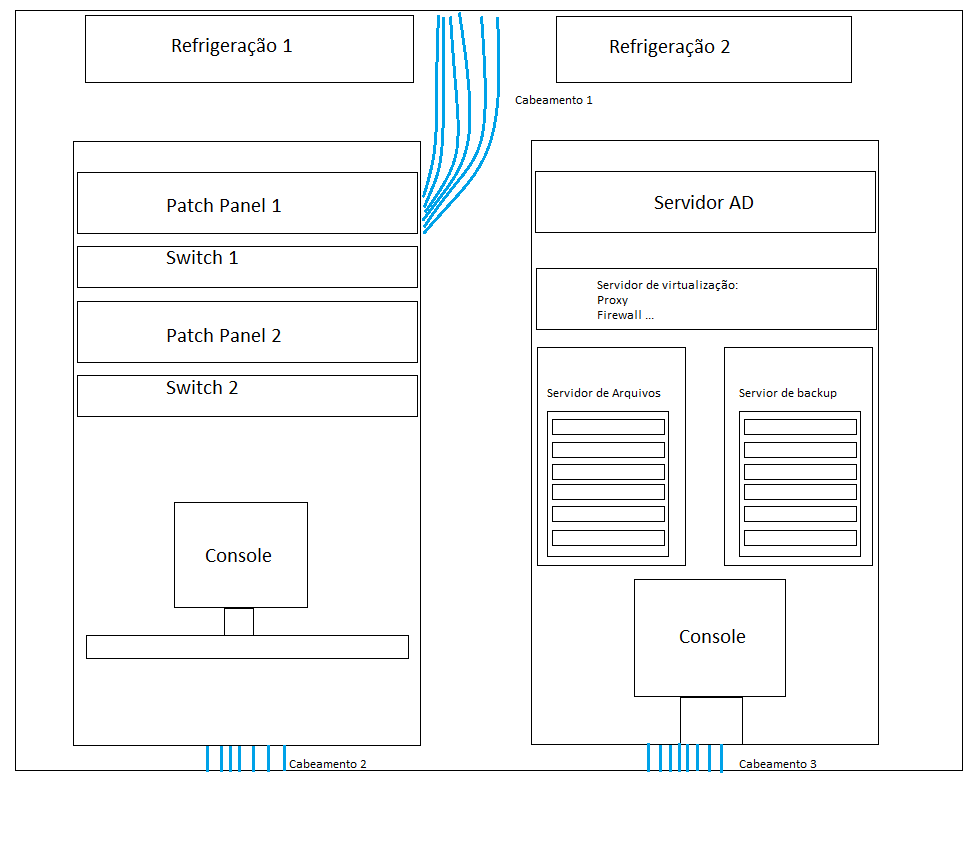
\includegraphics[width=\textwidth]{./imagens/datacenter.png}
	\caption{Exemplo de figura com escala horizontal}
	\label{fig:desenhoestrutura}
\end{figure}

	
\subsection{Topologia}
A topologia de redes física segundo \cite{forouzan2007} se refere à maneira pela qual uma rede é organizada fisicamente. Dois ou mais dispositivos se conectam a um link de comunicação; dois ou mais links formam uma topologia. Existe ainda o cenário de ser implementado uma topologia física e implantar uma topologia lógica diferente da Física. Na figura \ref{fig:tipos_topologias} pode ser visto alguns modelos de topologia, cada uma delas apresenta suas qualidades e defeitos, cabe a ao administrador definir qual melhor utilizar.

\begin{figure}[!htbp]
	\centering
	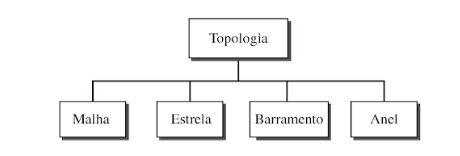
\includegraphics[width=\textwidth]{./imagens/tipos_topologia.png}
	\caption{Tipos de topologia}
	\cite{forouzan2007}
	\label{fig:tipos_topologias}
\end{figure}
 
\begin{figure}[!htbp]
 	\centering
 	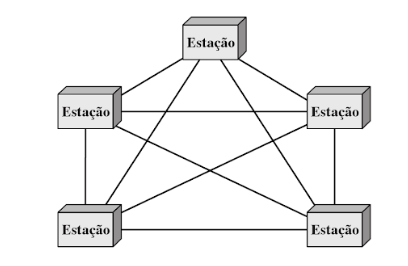
\includegraphics[width=\textwidth]{./imagens/malha.png}
 	\caption{Topologia Malha}
 	\cite{forouzan2007}
 	\label{fig:malha}
 \end{figure}

\begin{figure}[!htbp]
	\centering
	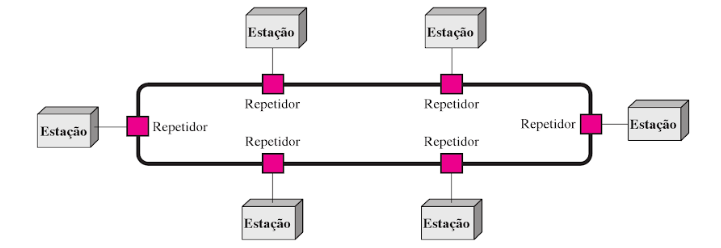
\includegraphics[width=\textwidth]{./imagens/anel.png}
	\caption{Topologia Anel}
	\cite{forouzan2007}
	\label{fig:anel}
\end{figure}
 
\begin{figure}[!htbp]
 	\centering
 	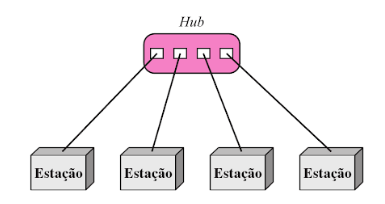
\includegraphics[width=\textwidth]{./imagens/estrela.png}
 	\caption{Topologia Estrela}
 	\cite{forouzan2007}
 	\label{fig:estrela}
 \end{figure}

\begin{figure}[!htbp]
	\centering
	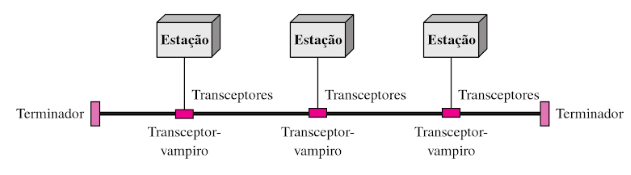
\includegraphics[width=\textwidth]{./imagens/barramento.png}
	\caption{Topologia Barramento}
	\cite{forouzan2007}
	\label{fig:barramento}
\end{figure}

De todas as topologias apresentada a mais ideal para o projeto seria topologia estrela conforme a Figura \ref{fig:estrela}. Segundo \cite{forouzan2007} a topologia em estrela cada dispositivo tem seu link ponto a ponto dedicado ligando apenas com o controlador central, em geral pode ser um Hub ou Switch. Os dispositivos não são ligados diretamente entre si. Diferentemente de uma topologia em malha, uma topologia em estrela não permite tráfego direto entre cada dispositivos. O Controlador atua como uma central telefônica: se um dispositivo quiser enviar dados para outro dispositivo, ele deve enviar ps dados primeiramente ao controlador que, então, os retransmite ao outro dispositivo. Em nosso cenário conforme descrito na Seção \ref{sec:Requisitos} o nosso controlado central será um Switch Cisco 2960L.
Esse Switch tem como as seguintes características são comutadores Gigabit Ethernet fixo e gerenciados de forma inteligente que fornecem comutadores de acesso de classe empresarial para filias, aplicativos "out-of-the-wiring closete" e implantações críticas de Internet das Coisas (Iot). Os Catalyst 2960-L Smart Managed Switches são switches seguros, confiáveis e de nível empresárias criados para implantações em pequenos escritórios. Esses switches podem ser configurados e gerenciados por meio de uma interface da Web on-box, permitindo aos clientes uma maneira rápida e confiável de colocar em funcionamento uma pequena filial ou uma rede de escritórios em poucos minutos. Esses switches também apresentam suporte CLI limitado para solução de problemas e monitoramento. Sendo ainda totalmente gerenciados que oferecem recursos avançados de Camada 2 e 3 básica, bem como energia Power Over Ethernet Plus (PoE +), oferecendo segurança de rede aprimorada, confiabilidade de rede e eficiência operacional. 
 	
\subsection{Encaminhamento}
Segundo \cite{pinheiro2015} os eletrodutos, recomenda-se o metálico rígido do tipo "pesado", e não a tubulação flexível. Devem ser utilizadas apenas curvas de 90\textdegree, do tipo suave. Não são permitidas curvas fechadas de 90\textdegree. Para as eletrocalhas, recomendam-se preferencialmente as do tipo lisa com tampa, porque evitam o acúmulo de sujeira. Não se instalam eletrocalhas acima de aquecedores, linhas de vapor ou incineradores. Ainda existem os ganchos que segura os eletrodutos que devem ser ganchos espaçados de no máximo 1,50m. Neles os cabos serão apoiados e travados por um processo que evite o seu esmagamento ou compreensão excessivas \cite{pinheiro2015}. 

\begin{figure}[!htbp]
	\centering
	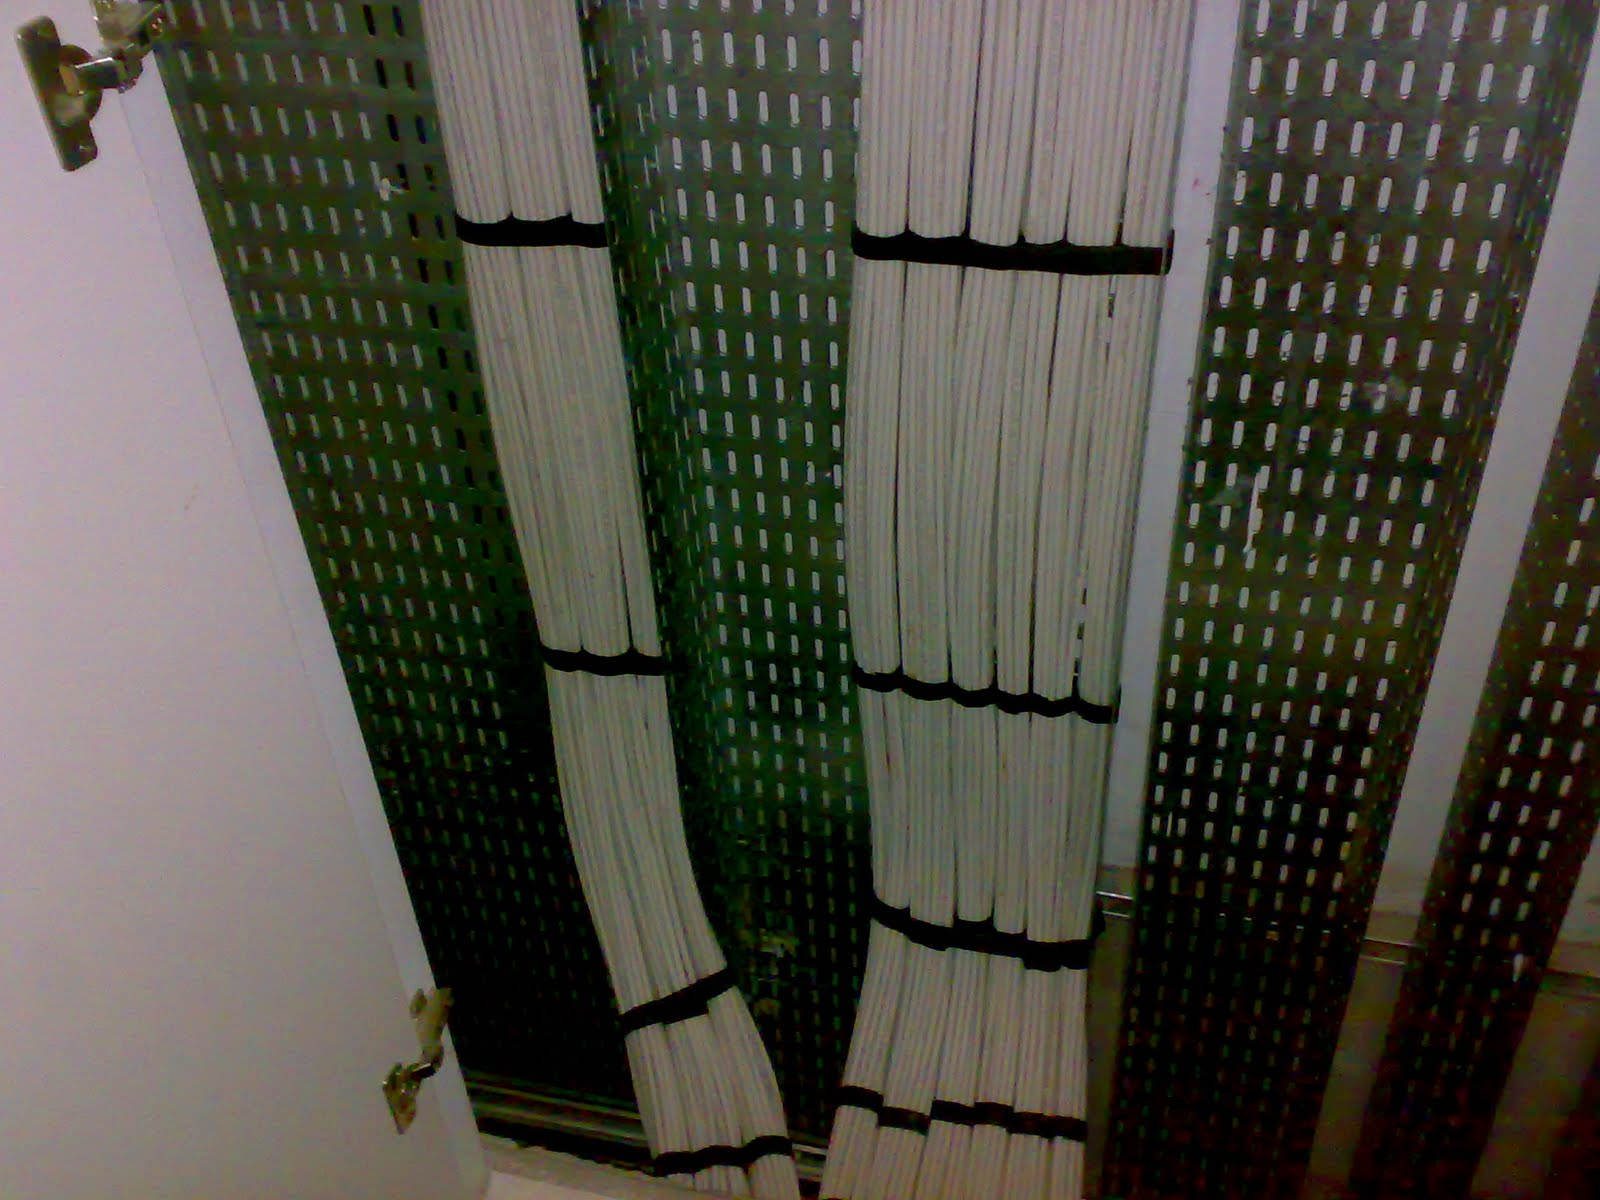
\includegraphics[width=\textwidth]{./imagens/organizacao_ideal.png}
	\caption{Organização ideal para data center.}
	\label{fig:cabeamento_ideal_datacenter}
\end{figure}

Em nosso projeto o será mais ideal uma calha de cabeamento que não deve ser complexo pois conforme a Figura \ref{fig:desenhoestrutura} os cabeamentos descem do forro, o que deve ser ajustado é colocar uma calha no teto até o chão que é de 3m e com isso ajustar no rack esquerdo no patch panel, isso pode ser visível na Figura \ref{fig:cabeamento_ideal_datacenter} , os cabos do forro podem ser organizado juntado eles com fita organizadoras, um belo exemplo de como deve ficar pode ser visto na Figura \ref{fig:cabeamento_ideal}.
 
\begin{figure}[!htbp]
	\centering
	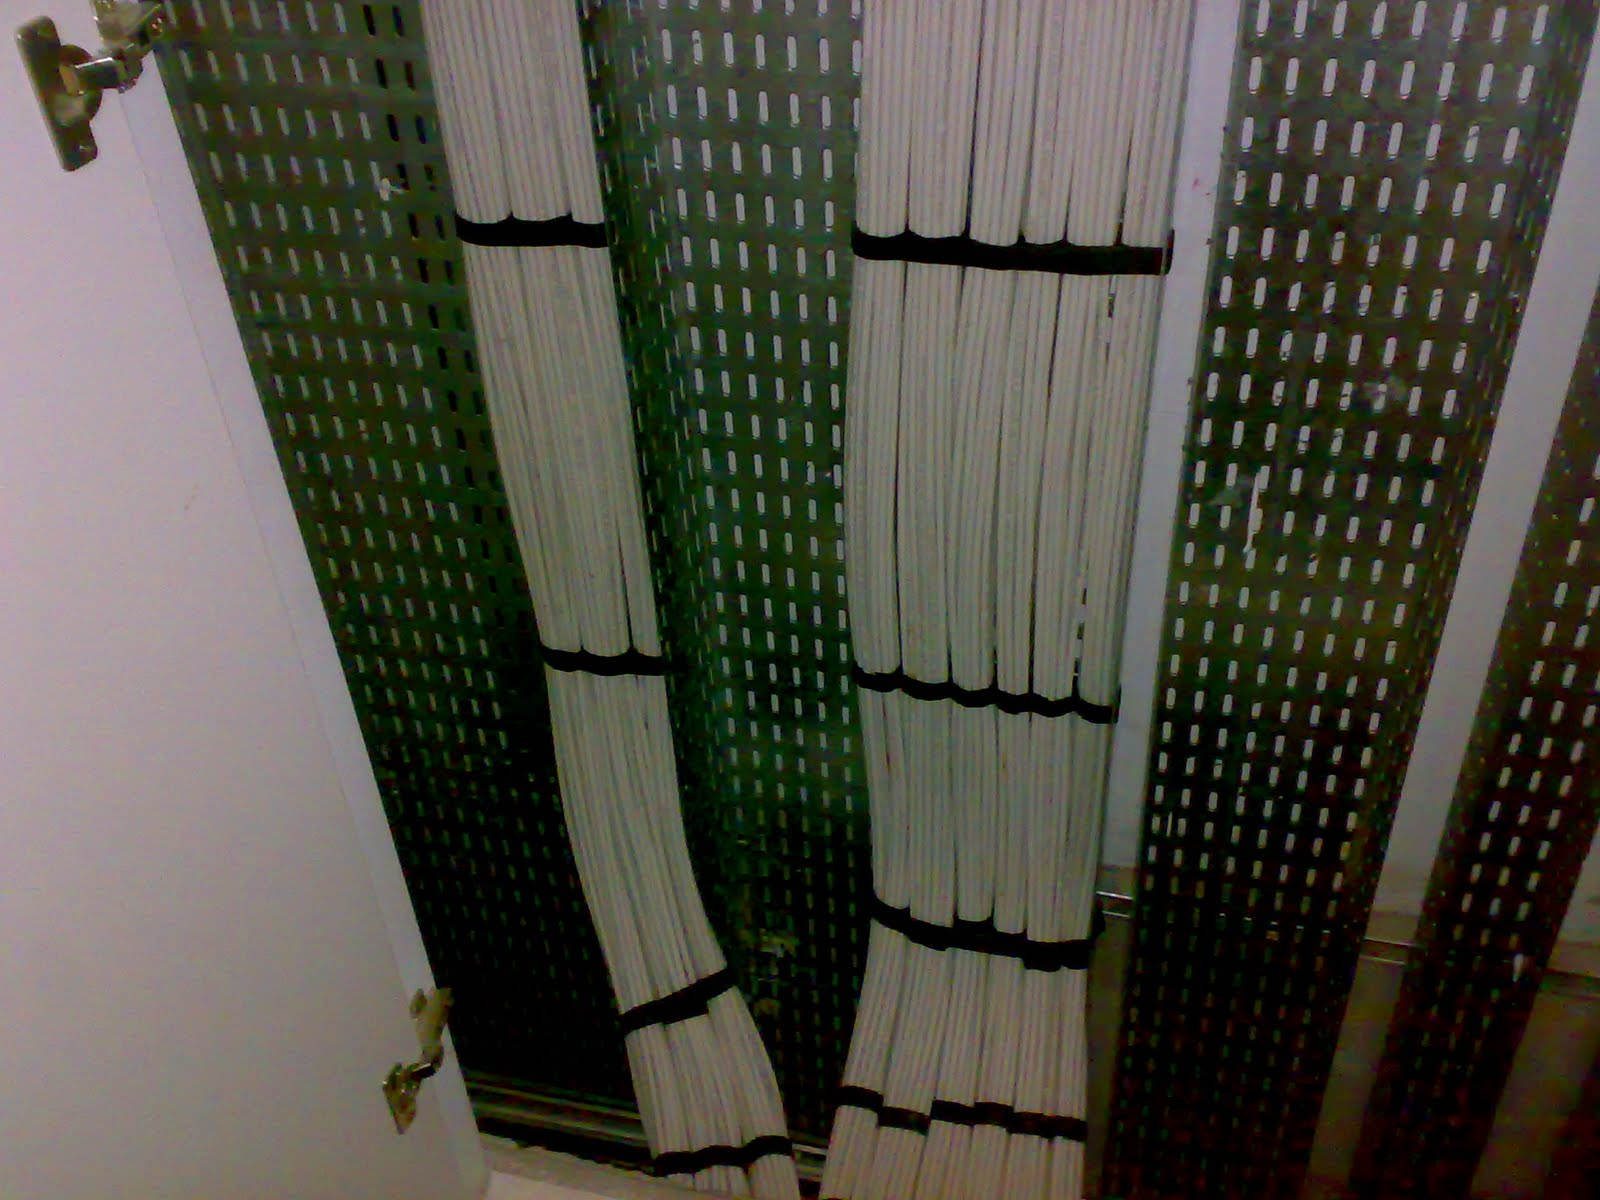
\includegraphics[width=\textwidth]{./imagens/organizacao_ideal.png}
	\caption{Organização ideal cabos + calhas.}
	\label{fig:cabeamento_ideal}
\end{figure}


\subsection{Identificação dos cabos}
O conceito de cabeamento e identificação dos componentes do cabeamento e o relacionamento desta com plantas da rede e relatórios são essenciais na administração do sistema. Casos como a identificação das falhas podem ser facilmente isolados quando se sabe que a tomada de telecomunicações que não funciona está conectada por um determinado cabo x que termina em uma conexão y. Desta tal situações, reconfigurar-se a conexão se torna um processo mais simples e rápido \cite{pinheiro2015}. Os ícones de identificadores são elementos de identificação do cabeamento, padronizados, colocados na parte frontal dos conectores fêmeas ou no patch panel. São utilizados para identificar pontos de rede e de telefonia, interligações de edifícios, etc., conforme a norma TIA-606, que regulamenta também a codificação de cores para identificar a aplicação de cada ponto, especificando os elementos que devem ser administrados, procedimentos de identificação e geração de documentação de cabeamento.  
No projeto atual o identificação mais ideal e prática é utilizar anilhas de identificação, conforme pode ser observado na Figura \ref{fig:anilhas_identificacao}. Como referido a identificação ajuda entender o que liga o que e resolver facilmente cabos com defeitos.

\begin{figure}[!htbp]
	\centering
	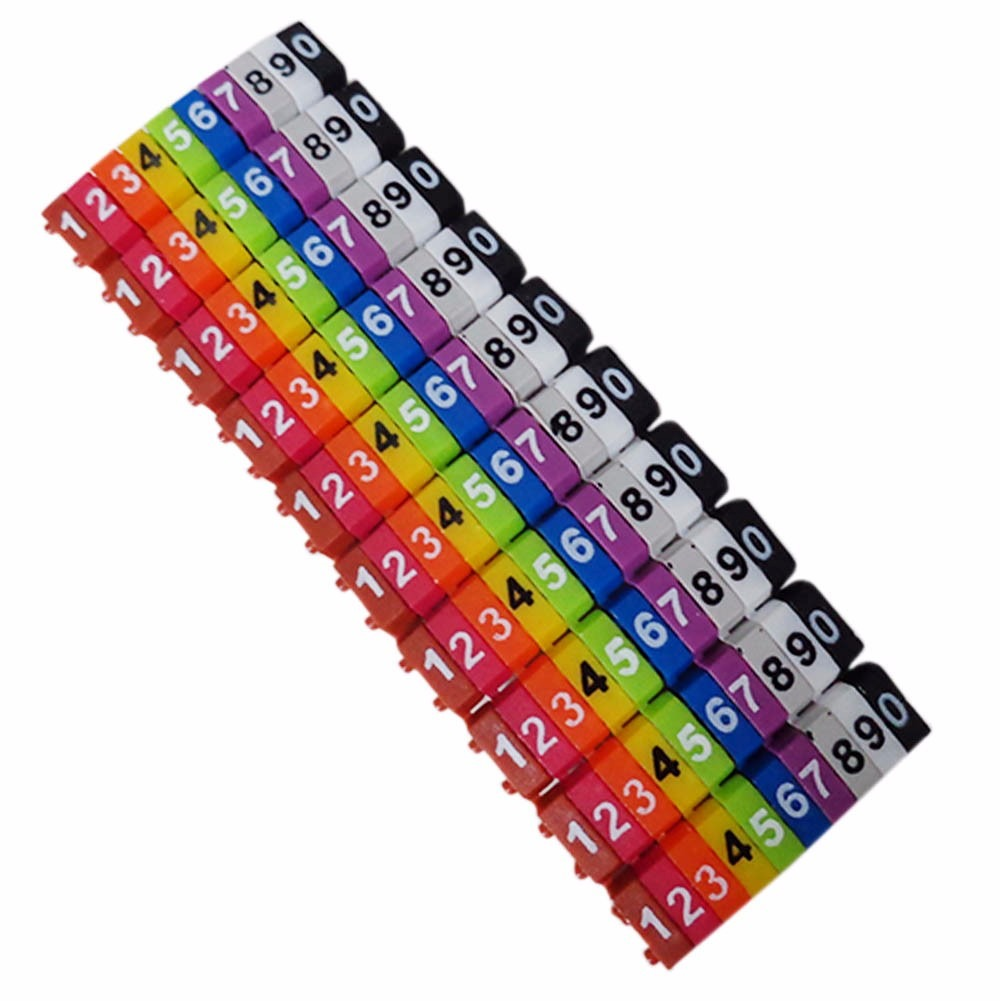
\includegraphics[width=\textwidth]{./imagens/identificador-de-cabos-anilhas.png}
	\caption{Anilhas de identificação.}
	\label{RV Cabeamento Estruturado}
	\label{fig:anilhas_identificacao}
\end{figure} 

\section{Plano de certificação}\label{sec:plano_certificacao}
Segundo \cite{Samuel} o processo de certificação do cabeamento estruturado de uma rede, sendo composta por cabos de par-trançados ou fibras ópticas, requer os equipamento especializados e envolve uma série de parâmetros determinados pela normas \textbf{ANSI/TIA-568-C /b (2009)}. Os certificadores de cabos da \textbf{Fluke Networks}. Esses certificadores de cabos pode ser vistos na Figura \ref{fig:fluke_networks}, sendo eles de referência mundial.

\begin{figure}[!htbp]
	\centering
	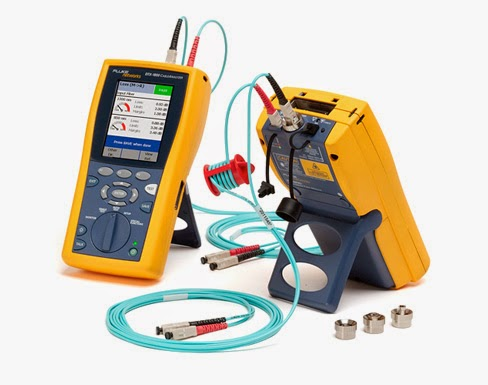
\includegraphics[width=\textwidth]{./imagens/fluke.png}
	\caption{Fluke Networks.}
	\label{fig:fluke_networks}
	\cite{Samuel}
\end{figure} 

Para a cerificação são exigidos vários testes pela norma, como: 
\begin{itemize}
\item Configuração de Terminação (Wire Map);
\item Comprimento do Cabo;
\item Perda de Inserção (Atenuação);
\item Perda de Retorno (Impedância);
\item Paradiafonia (NEXT), PS-NEXT, ELNEXT e PS-ELNEXT;
\item Relação Atenuação/Paradiafonia (ACR);
\item Atraso de Propação (Delay);
\item Desvio no Atraso de Propagação (Delay Skew).
\end{itemize}

O teste de mapeamento de fios é o mais simples dos testes onde consiste em assegurar que a sequências de fios nos conectores RJ-45 dos cabos de par-trançados estejam em conformidade com os padrões \textbf{T568A} ou \textbf{T568B}, onde isso pode ser observado na Figura \ref{fig:mapeamento_de_fios}.

\begin{figure}[!htbp]
	\centering
	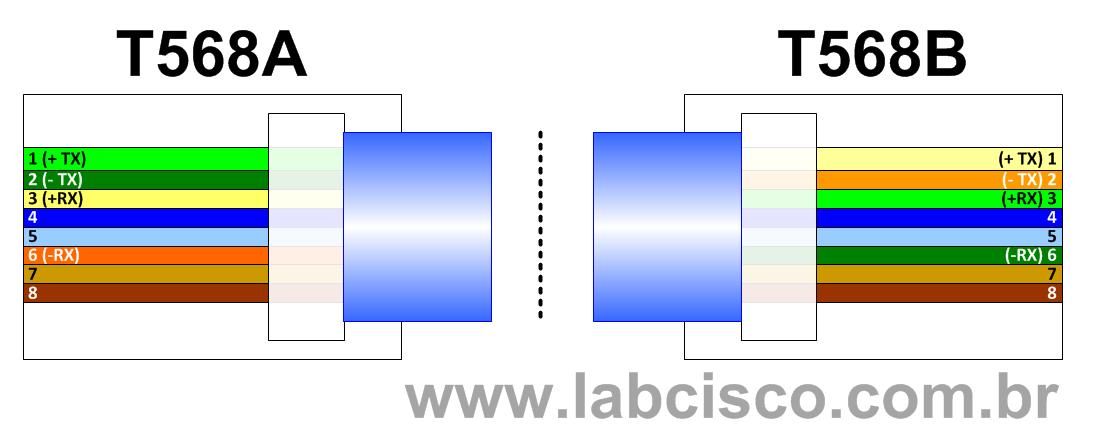
\includegraphics[width=\textwidth]{./imagens/mapeamento_de_fios.png}
	\caption{Padrões T568A e T568B.}
	\label{fig:mapeamento_de_fios}
	\cite{Samuel}
\end{figure} 

A organização dos demais parâmetros nas seguintes categorias:
\begin{itemize}
\item Diafonia
\item Impedância
\item Atenuação
\end{itemize}

A Difonia ou também conhecida como linha cruzada (crosstalk) ocorre quando um determinado par de fios gera interferência em outros par nas proximidades, seja no mesmo cabo ou em outros \cite{Samuel}.
A Impedância é a medida da resistência (em ohms $\omega$) que deve ser uniforme ao longo do cabo e conectores. A norma utilizada é a ANSI/TIA-568-C recomenda cautela na tração excessiva aos condutores, emendas desnecessárias e torcimentos dos cabos pois essas ações impactam negativamente no valor de impedância, cujo limite de tolerância é de 15% \cite{Samuel}.
E a atenuação é expressa em dB e representa a redução da amplitude do sinal ao longo do cabo (perda). Pode-se degradar em frequências mais altas, motivo pelo qual os equipamentos fazem sua medição em diferentes frequências que podem variar dos 64kHz até 100MHz (no cabo Cat5e) ou mais em outras categorias \cite{Samuel}.

Conforme apresentado como é o plano de certificações e o que deve ser analisado e as categorias que pode interferir sem seu mal funcionamento será necessário o equipamento da Fluke Microscanner2, o mesmo pode ser observado na Figura \ref{fig:fluke-microscanner2}. Verificado no mercado a existência de vários modelos da Fluke e preços o mais acessível e de ótimo custo benefício seria o Fluke Microscanner2, nesse equipamento ele apresenta as seguintes características de certificação:
\begin{itemize}
	\item Verifica os serviços disponíveis (10/100/1000 Ethernet, telefonia e POE);
	\item Mostra comprimento de cabo, pinagem, ID de cabo e distância até a falha em uma tela;
	\item Testa todos os tipos de mídia comuns, incluindo RJ-11, RJ-45, Coaxial sem necessidade de adaptadores;
	\item Tela grande e retro-iluminada torna os resultados claros em qualquer ambiente de trabalho;
	\item Capa emborrachada aumenta a durabilidade e resistência do equipamento.
\end{itemize}

\begin{figure}[!htbp]
	\centering
	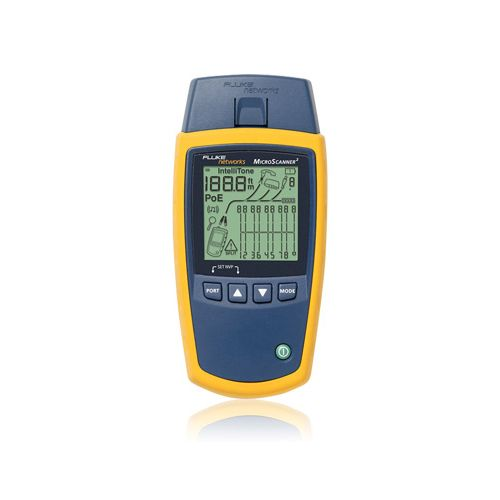
\includegraphics[width=\textwidth]{./imagens/fluke-microscanner2.png}
	\caption{Fluke Microscanner2.}
	\label{fig:fluke-microscanner2}
\end{figure} 

Neste equipamento não há suporte para fibras ópticas, mas no nosso cenário empresarial não a necessidade desse tipo de verificação, pois o único cabo de fibra que chega até a sede é a de internet, os demais cabos são UTP.  

\section{Plano de manutenção}
As revisões dos cabos serão feitas em duas etapas diferentes. A primeira delas será verificação dos cabos de redes e conexões dentro do data center, testando todos os cabos com o equipamento Fluke Microscanner2, validando se ainda os cabos estão em qualidade aceitável, conforme descrito na Seção \ref{sec:plano_certificacao}. Já na segunda etapa é a vez dos cabos dos colaboradores, verificando se não estão inoxidável e se também estão dentro dos padrões solicitados. Essas revisões serão 2 vezes ao ano no data center e 3 vezes ao ano nos colaboradores o dia da semana ideal para isso é sábado ou domingo, pois esses dias não há colaboradores trabalhando e fica mais fácil verificar os equipamentos, já no data center será feito uma redundância dos serviços para que quando for realizar a certificação dos cabos os serviços não parem.

\subsection{Plano de expansão}
A expansão dos pontos e máquinas não deve ser grande, mas os planos desse artigo é prever o crescimento da rede, então conforme a Figura \ref{fig:cabeamento_ideal_datacenter} do data center, o rack da esquerda possui espaço para mais switch e patch panel, diminuindo o espaço do console, ou até mesmo tirando ele colocando em outro menor. Pensando nessa expansão é possível colocar outro switch 2 de 96 portas essa expansão seria a um longo prazo até isso se concluir, visto que o no cenário atual com dois switch de 48 portas, dando total de 96 portas já é mais que o suficiente já que o parque de máquinas atuais é de cercas de 60 equipamentos. Já no rack direito onde fica servidores de aplicação, arquivos e backup pode-se aumentar o armazenamento das fitas ganhando um tempo considerável até alguma futura mudança de aumento de racks que isso já iria ser necessário outro projeto. Essa solução atual já certifica um bom funcionamento para um longo prazo.

\section{Risco}
Enumerar e explicar os riscos do projeto.

\section{Orçamento}
O orçamento será com base no que foi levantado na Seção \ref{sec:Requisitos}, na Tabela  é apresentado os preços de cada equipamento:
\begin{table}[!htbp]
	\centering
	\begin{tabular}{|l|l|l|l|}
		\cline{1-4}
		\textbf{Componentes}        & \textbf{Qts.} &  Preço Uni.          & Total \\
		\cline{1-4}
		Patch panel (furukawa GIGALAN CAT.6 de 24 portas) & 4  & 699,99R\$ 			      &  2799,96R\$ \\
		\cline{1-4}
		Switch gerenciável (Cisco 2960L)                  & 2  & 15.000,00R\$ 			  & 30.000,00R\$  \\
		\cline{1-4}
		Access Points 	   (Cisco Air-lap 1141n-a-k) 	  & 4  & 550,00R\$    			  & 1100,00R\$  \\
		\cline{1-4}
		Servidor Monitoramento SNMP 	 				  & 1  & 0R\$         			  & 0R\$  \\	
		\cline{1-4}
		Patch Cord Cat.6  3m (Furukawa)	   				  & 96 & 11,20R\$  		          & 1075,2R\$   \\
		\cline{1-4}
		Patch Cord Cat.6  5m (Furukawa)	   				  & 96 & 20 9R\$ 		  		  & 2006,4R\$  \\
		\cline{1-4}
		Fluke Microscanner2	   							  & 1  & 5.790R\$ 		  		  & 5.790R\$ \\
		\cline{1-4}
		Total: 											  &    &                          &  42.771,56R\$ \\
		\cline{1-4}
	\end{tabular}
	\caption{Tabela para requisitos do projeto}\label{tab:orcamento}
\end{table}

Como pode ser observado o servidor SNMP não ira ter custo pois como será utilizado um ferramenta \textit{open source} virtualizada. Os demais valores forem coletados em alguns sites, e podem ter variações com o passar do tempo. 

\section{Recomendações}
Observações e recomendações para o cliente.

\section{Referências bibliográficas}
\renewcommand\refname{} %%Referências bibliográficas}  
\bibliographystyle{ieeetr}
\bibliography{referencias}  

\end{document}